\begin{titlepage}
\begin{center}

\includegraphics[scale=0.15]{Documents/niser.png}
\line(1,0){300}\\
[2mm]
\begin{large}
\textbf{\huge Counter Circuits}\\ 
\end{large}
\line(1,0){150}\\
[5cm]
\large MAITREY SHARMA\\
\small (1911093)\\
[4.5cm]
Second Year Integrated M.Sc.\\
\textbf{School of Physical Sciences}\\
\textbf{National Institute of Science Education and Research, Bhubaneshwar}\\
\small March 31, 2021
\end{center} 
\end{titlepage}
\newpage
\section{Aim}
\noindent
To construct and study the operations of the following circuits:
\begin{enumerate}
    \item A 4-bit binary ripple Up-counter
    \item A 4-bit binary ripple Down-counter
    \item A Mod-12 counter
    \item A Ring counter
\end{enumerate}
\section{Apparatus}
\noindent Resistors, Digital ICs (JK flip-flop (7476), OR (7432), AND (7408), NAND (7420), NOT (7404)), DC Power Supply, Function Generator, Oscilloscope, LEDs, Connecting wires, Breadboard.
\section{Theory}
\noindent
An \textbf{\emph{electronic counter}} is a sequential logic circuit which has a clock input signal and a group of output signals that represent an integer \emph{counts} value. Basically, a counter is a device which stores (and sometimes displays) the number of times a particular event or process has occurred, often in relationship to a clock.
\newline
\noindent
\textbf{\emph{Binary counters}} are one of the type of electronic counters which use \emph{counting} in binary (that is base 2) instead of the usual decimal (base 10). Binary Counters can be constructed using flip-flops and the output is usually a direct representation of the counts. Once a clock pulse is fed into a counter circuit, the flip-flops present inside the counter undergo change of state in such a manner that the binary number stored in the flip-flops represents the number of pulses applied at input. When clock 
pulses are applied to a counter, the counter progresses from one state to another and the 
final output of the flip-flop in the counter indicates the pulse count.
\newline
\noindent
On basis of clock signal received by the flip-flops in the counters, they can be of two types: synchronous and asynchronous. If the flip-flops do not receive the same clock signal, then that counter is called as \textbf{\emph{Asynchronous counter}}. The output of system clock is applied as clock signal only to first flip-flop. The remaining flip-flops receive the clock signal from output of its previous stage flip-flop. Hence, the outputs of all flip-flops do not change at the same time. The asynchronous counters are also called \textbf{\emph{ripple counters}}.
\newline
\noindent
If all the flip-flops receive the same clock signal, then that counter is called as \textbf{\emph{Synchronous counter}}. Hence, the outputs of all flip-flops change at the same time.
\newline
\noindent
An $n$-bit binary counter consists of $n$ flip-flops. If the counter counts from $0$ to $2^N - 1$ then it is called as \textbf{\emph{binary up counter}}. Similarly, if the counter counts down from $2^N - 1$to $0$, then it is called as \textbf{\emph{binary down counter}}. This can be easily understood by taking note of the fact that the flip-flops have two states.

\par
\noindent
Consider the following 4-\emph{bit} ripple up-counter:
\begin{center}
    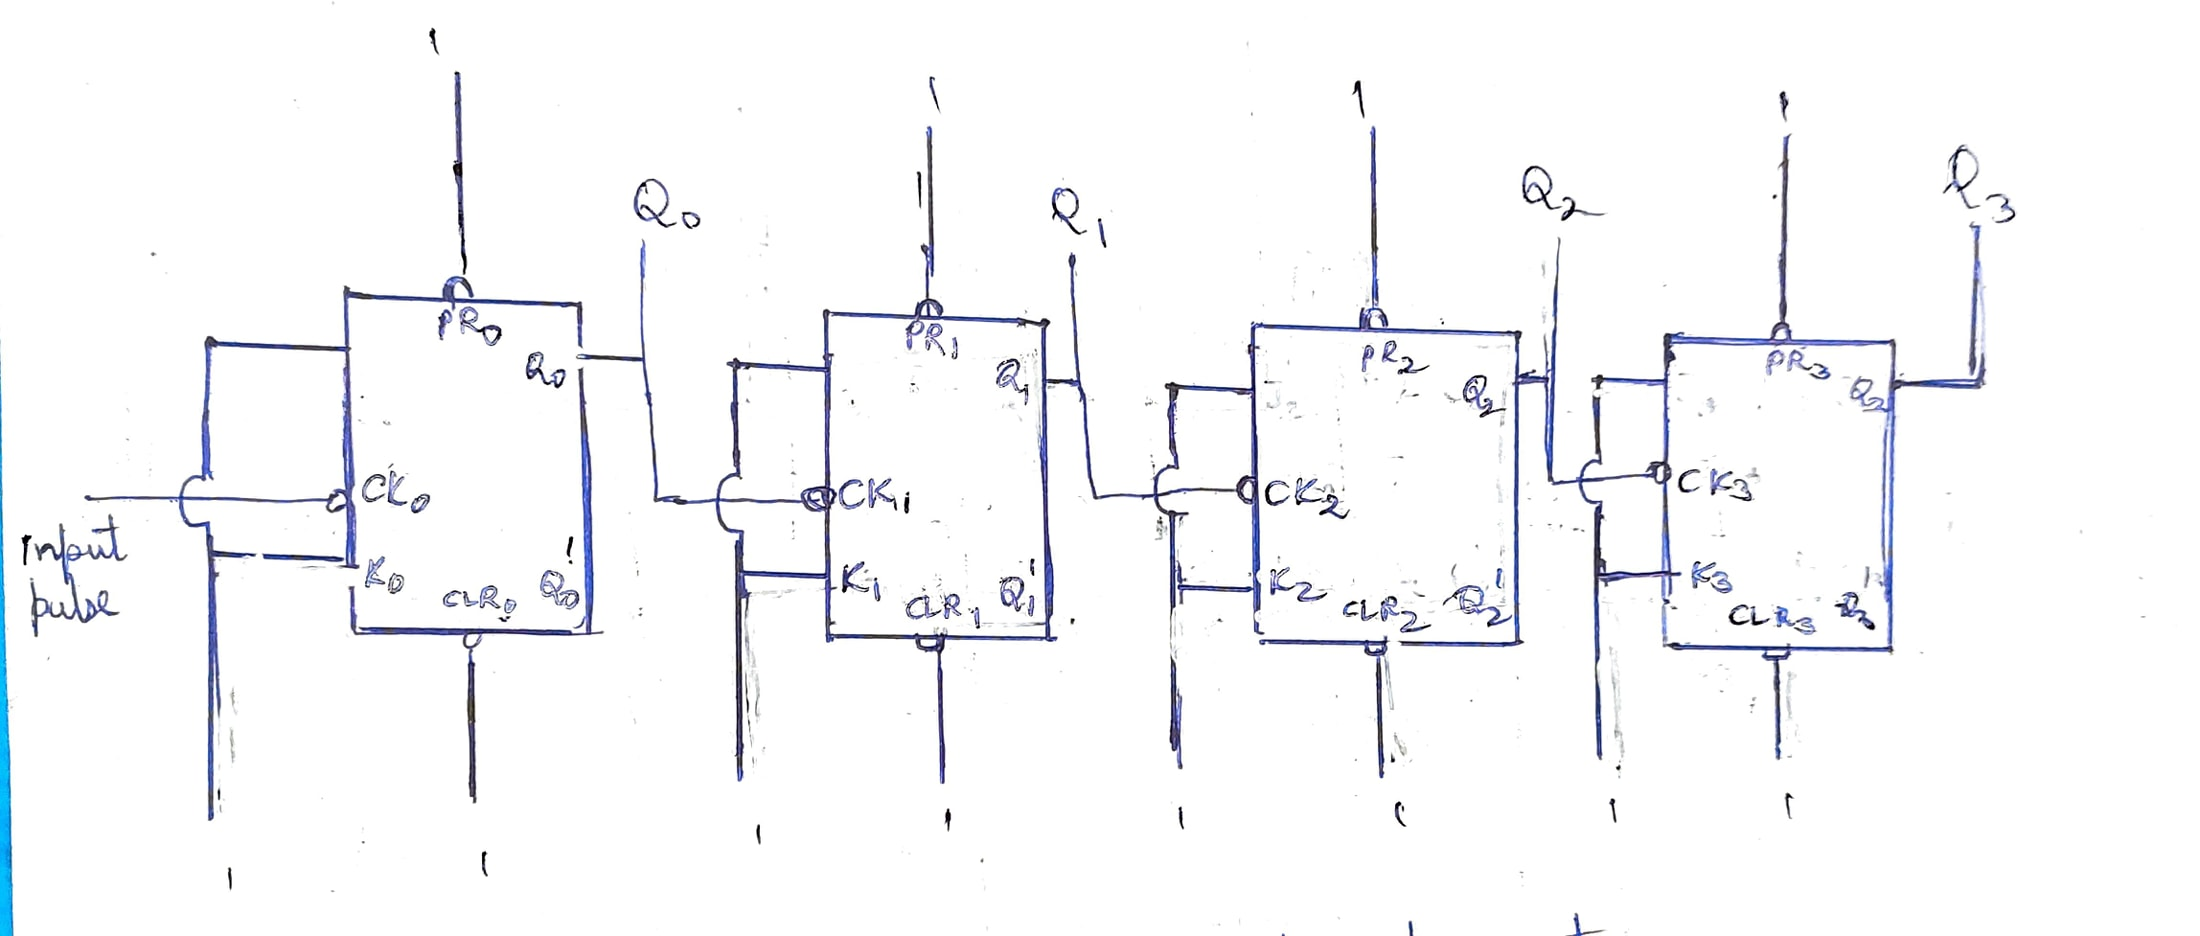
\includegraphics[scale = 0.15]{Figures/upcount_1.jpg}
\end{center}
\noindent
It is implemented using 4 JK flip-flops and it can be noticed that the normal output of each flip-flop is connected to the clock input of next flip-flop, thus making it asynchronous. Similarly, a 4-\emph{bit} ripple down counter can be constructed in a similar manner as follows:
\begin{center}
    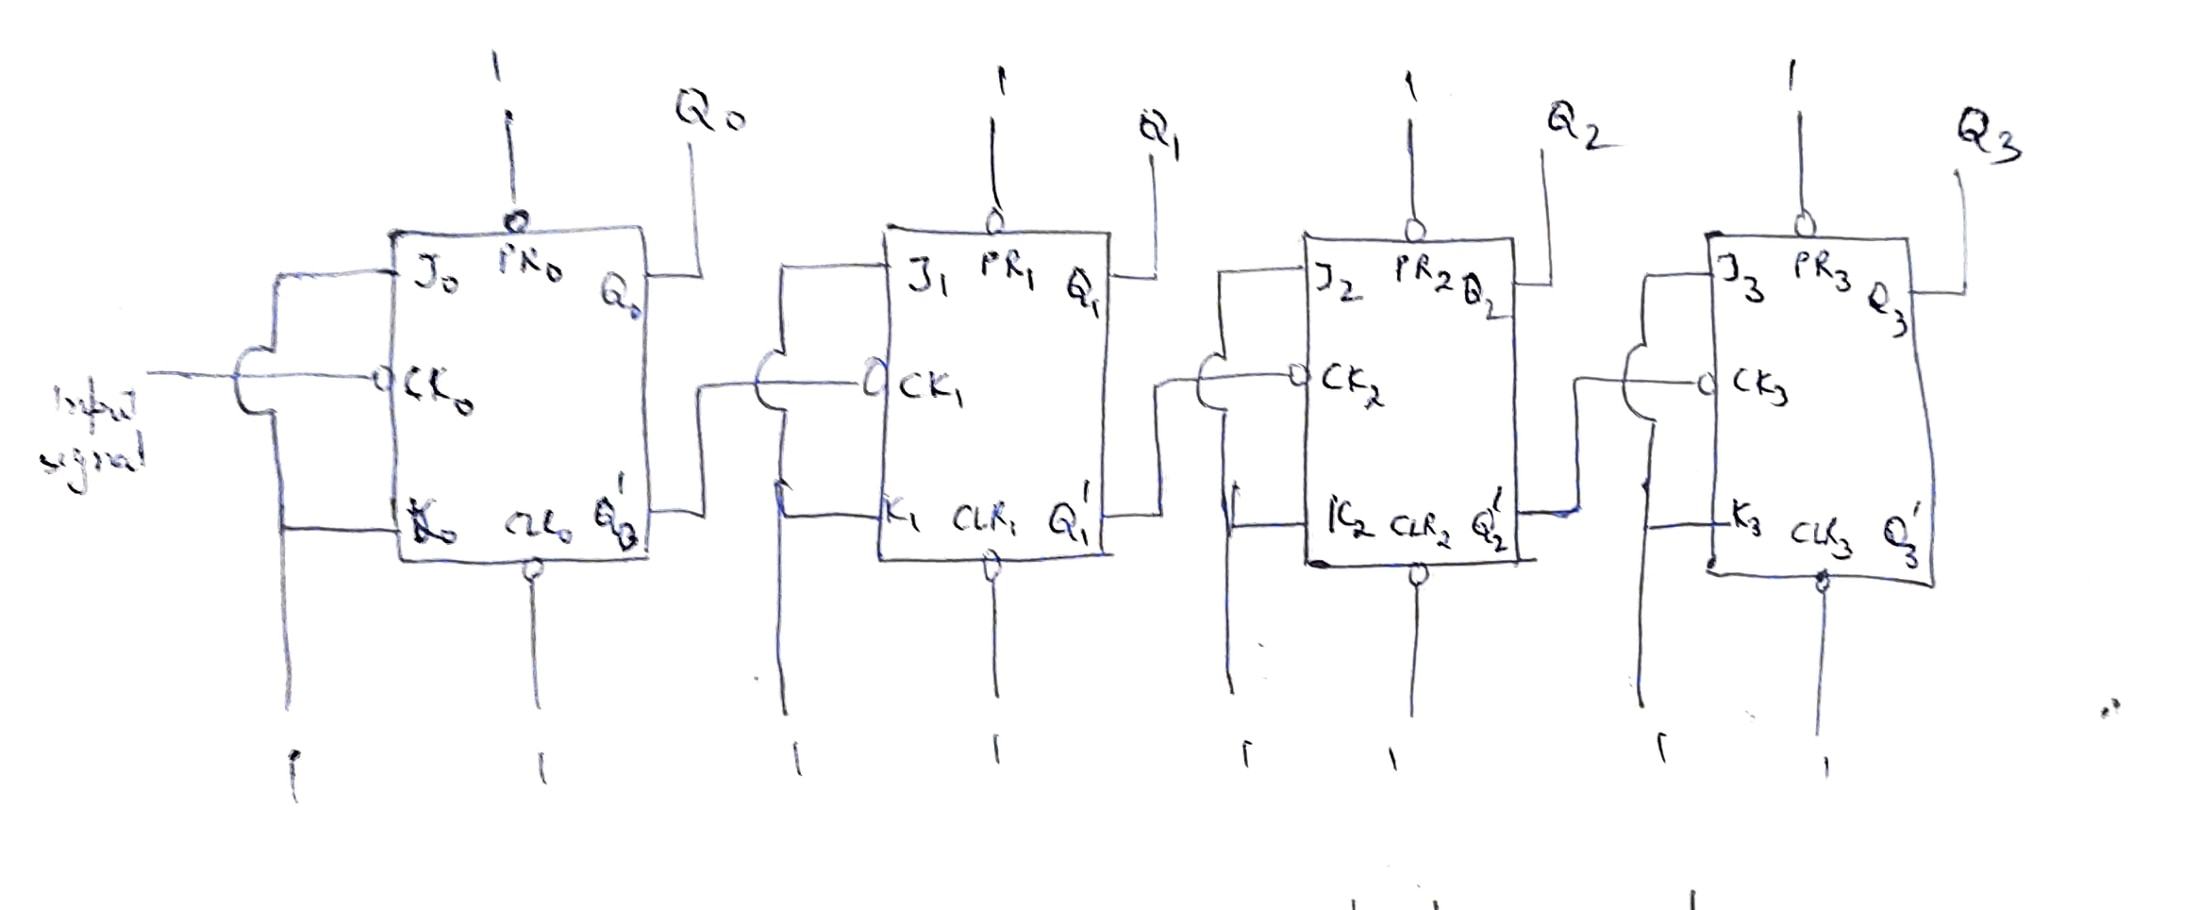
\includegraphics[scale = 0.15]{Figures/downcount_1.jpg}
\end{center}
\noindent
Here too, the inputs in the subsequent flip-flops are being fed are actually the outputs of the previous flip-flops. The only difference is that in down counters, the subsequent inputs are taken from the complementary output.
\newline
We can actually extend the concept of binary counters to count to any number (depending on the \emph{bits} available.). Therefore, we can design the so called, \textbf{\emph{Modulo-$n$}} counters, which should count till $n$. To design a modulo-$n$ counter, we will have to employ a modulo-$m$ counter where $m$ is the minimum exponent of 2 greater than $n$. For example, to construct a modulo-12 counter, we need a modulo-16 counter, which will skip the rest counts once the desired count is reached. The circuit diagram for a modulo-12 counter is as follows:
\begin{center}
    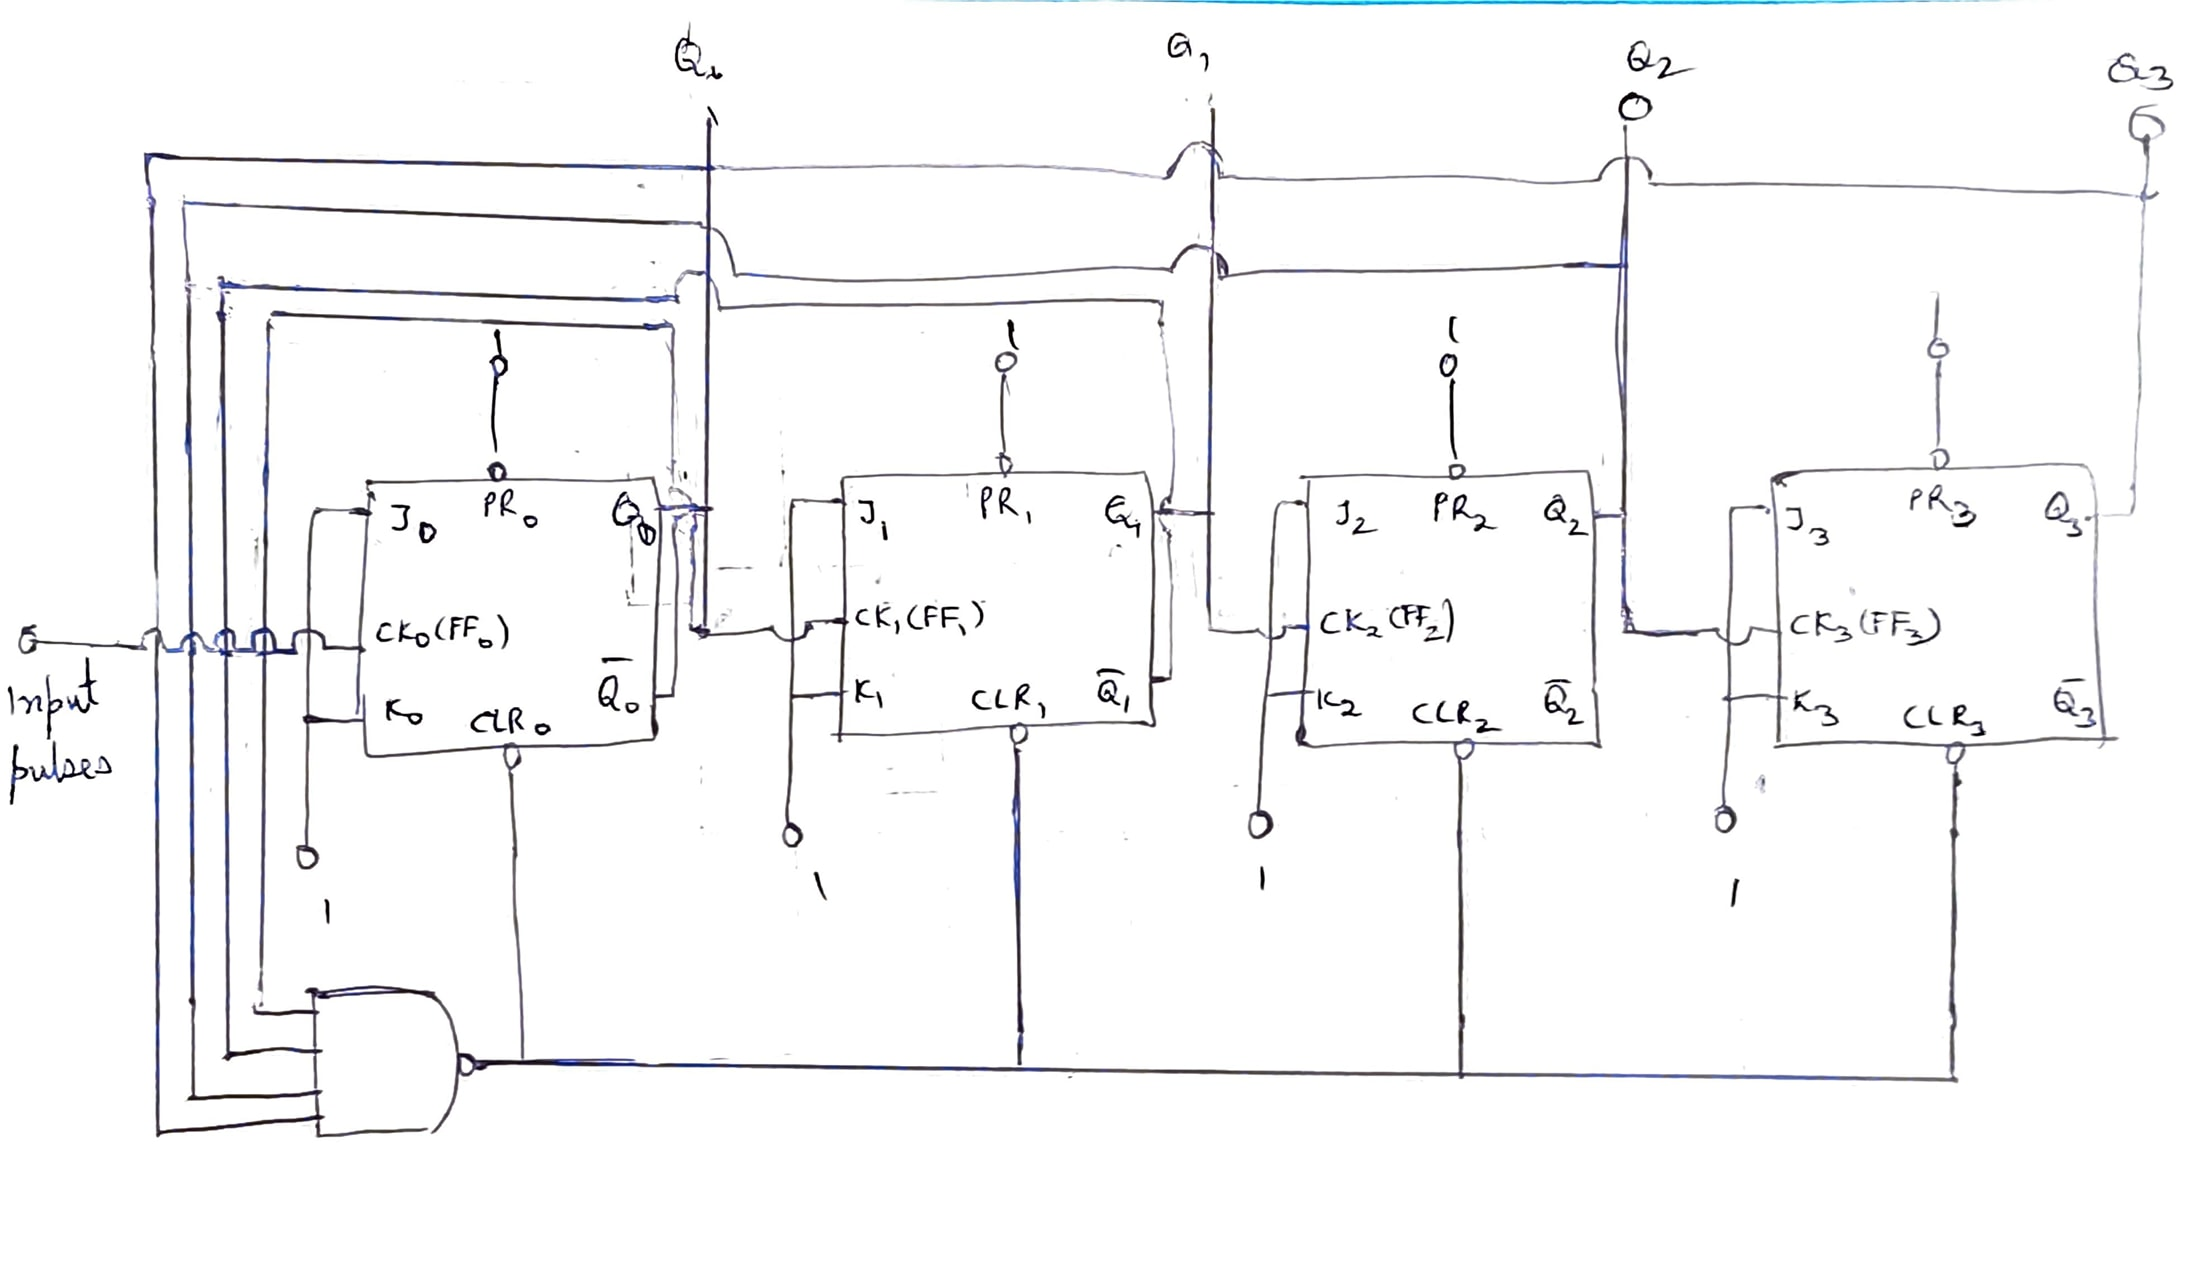
\includegraphics[scale = 0.2]{Figures/mod12_1.jpg}
\end{center}
Lastly, a \textbf{\emph{Ring Counter}} can be used to provide a sequence of equally spaced timing pulses. In ring counters, the output of the last flip-flop fed to the input of the first, making a \emph{circular} or \emph{ring} structure. The circuit diagram is as follows:
\begin{center}
    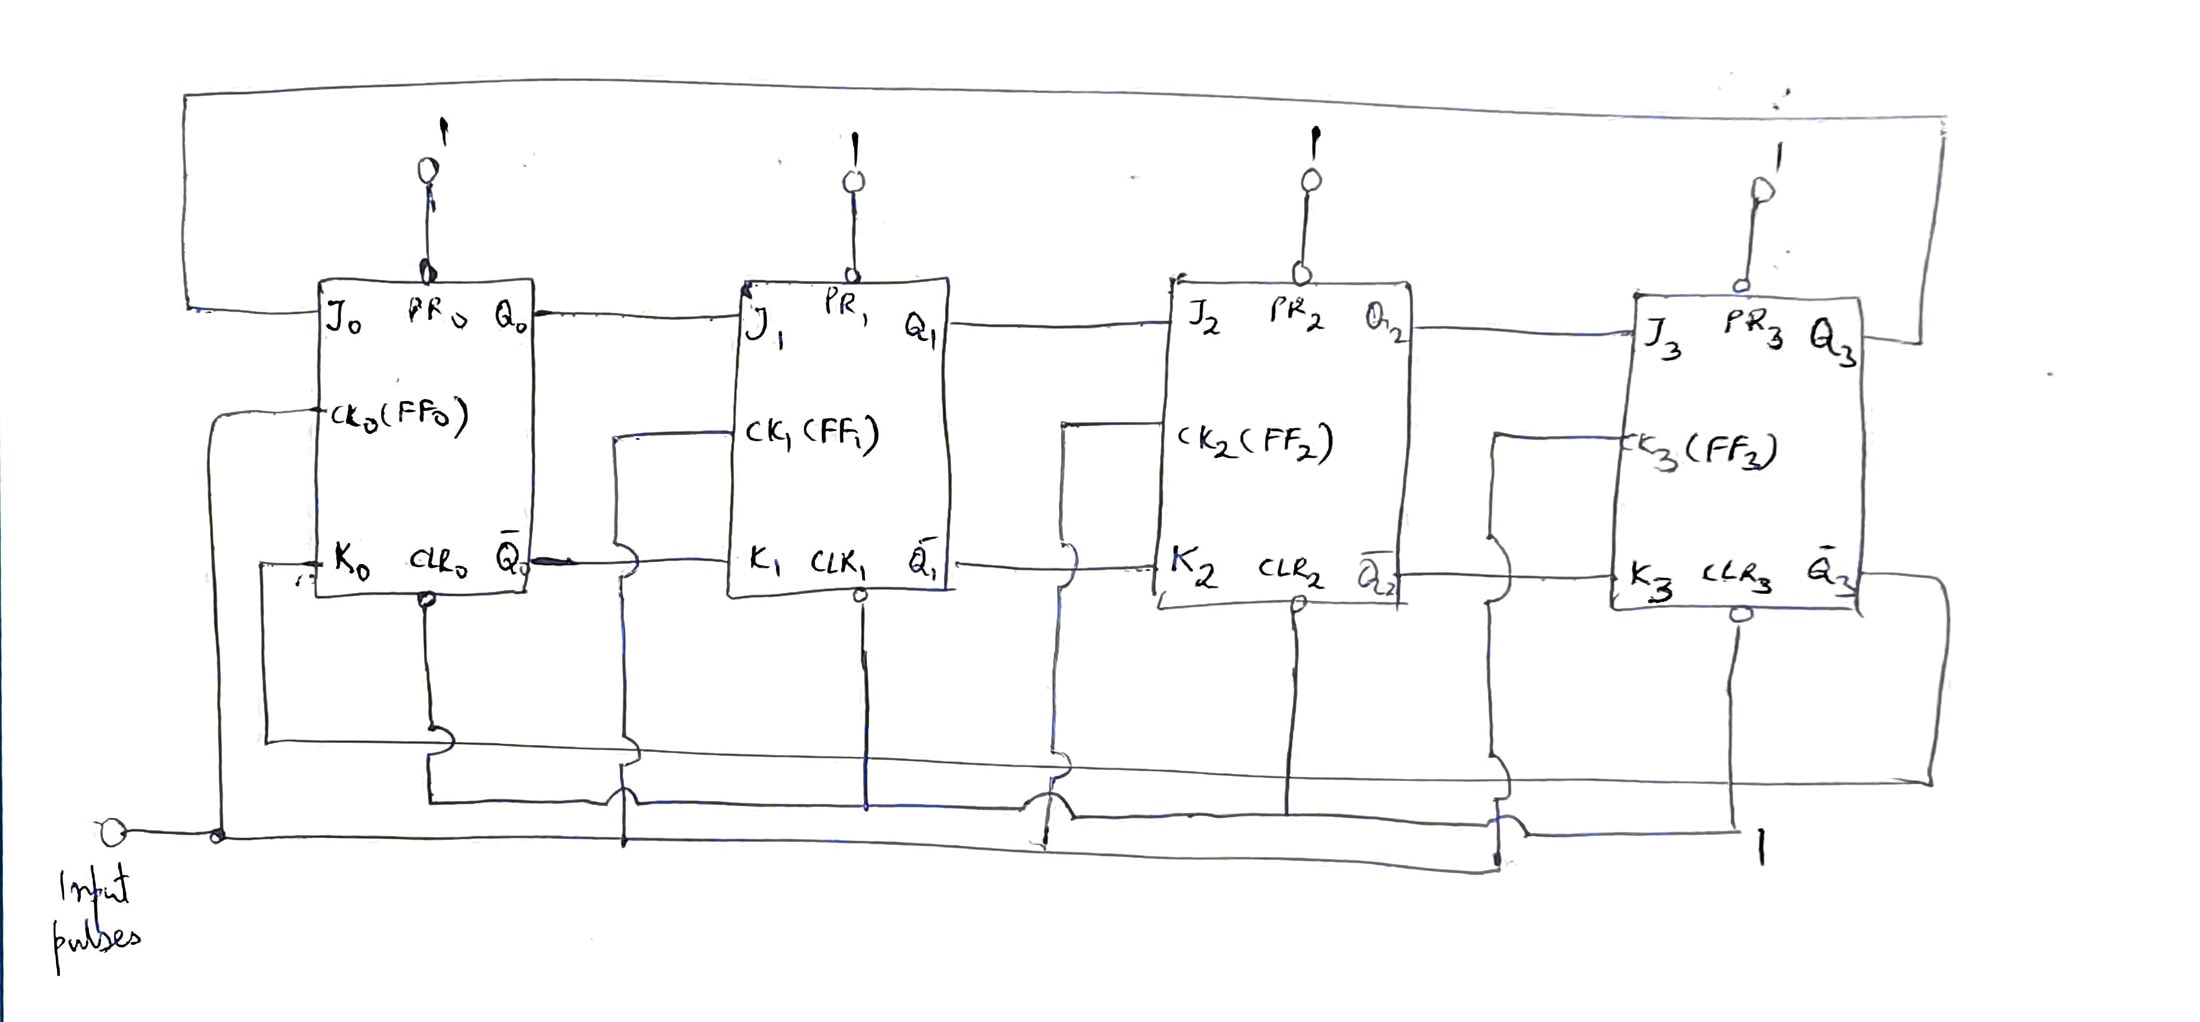
\includegraphics[scale = 0.2]{Figures/1617014472077.jpg}
\end{center}
\section{Observations}
\begin{center}
    \textbf{Characteristic table of 4-bit binary ripple up-counter}
\end{center}
\begin{center}
    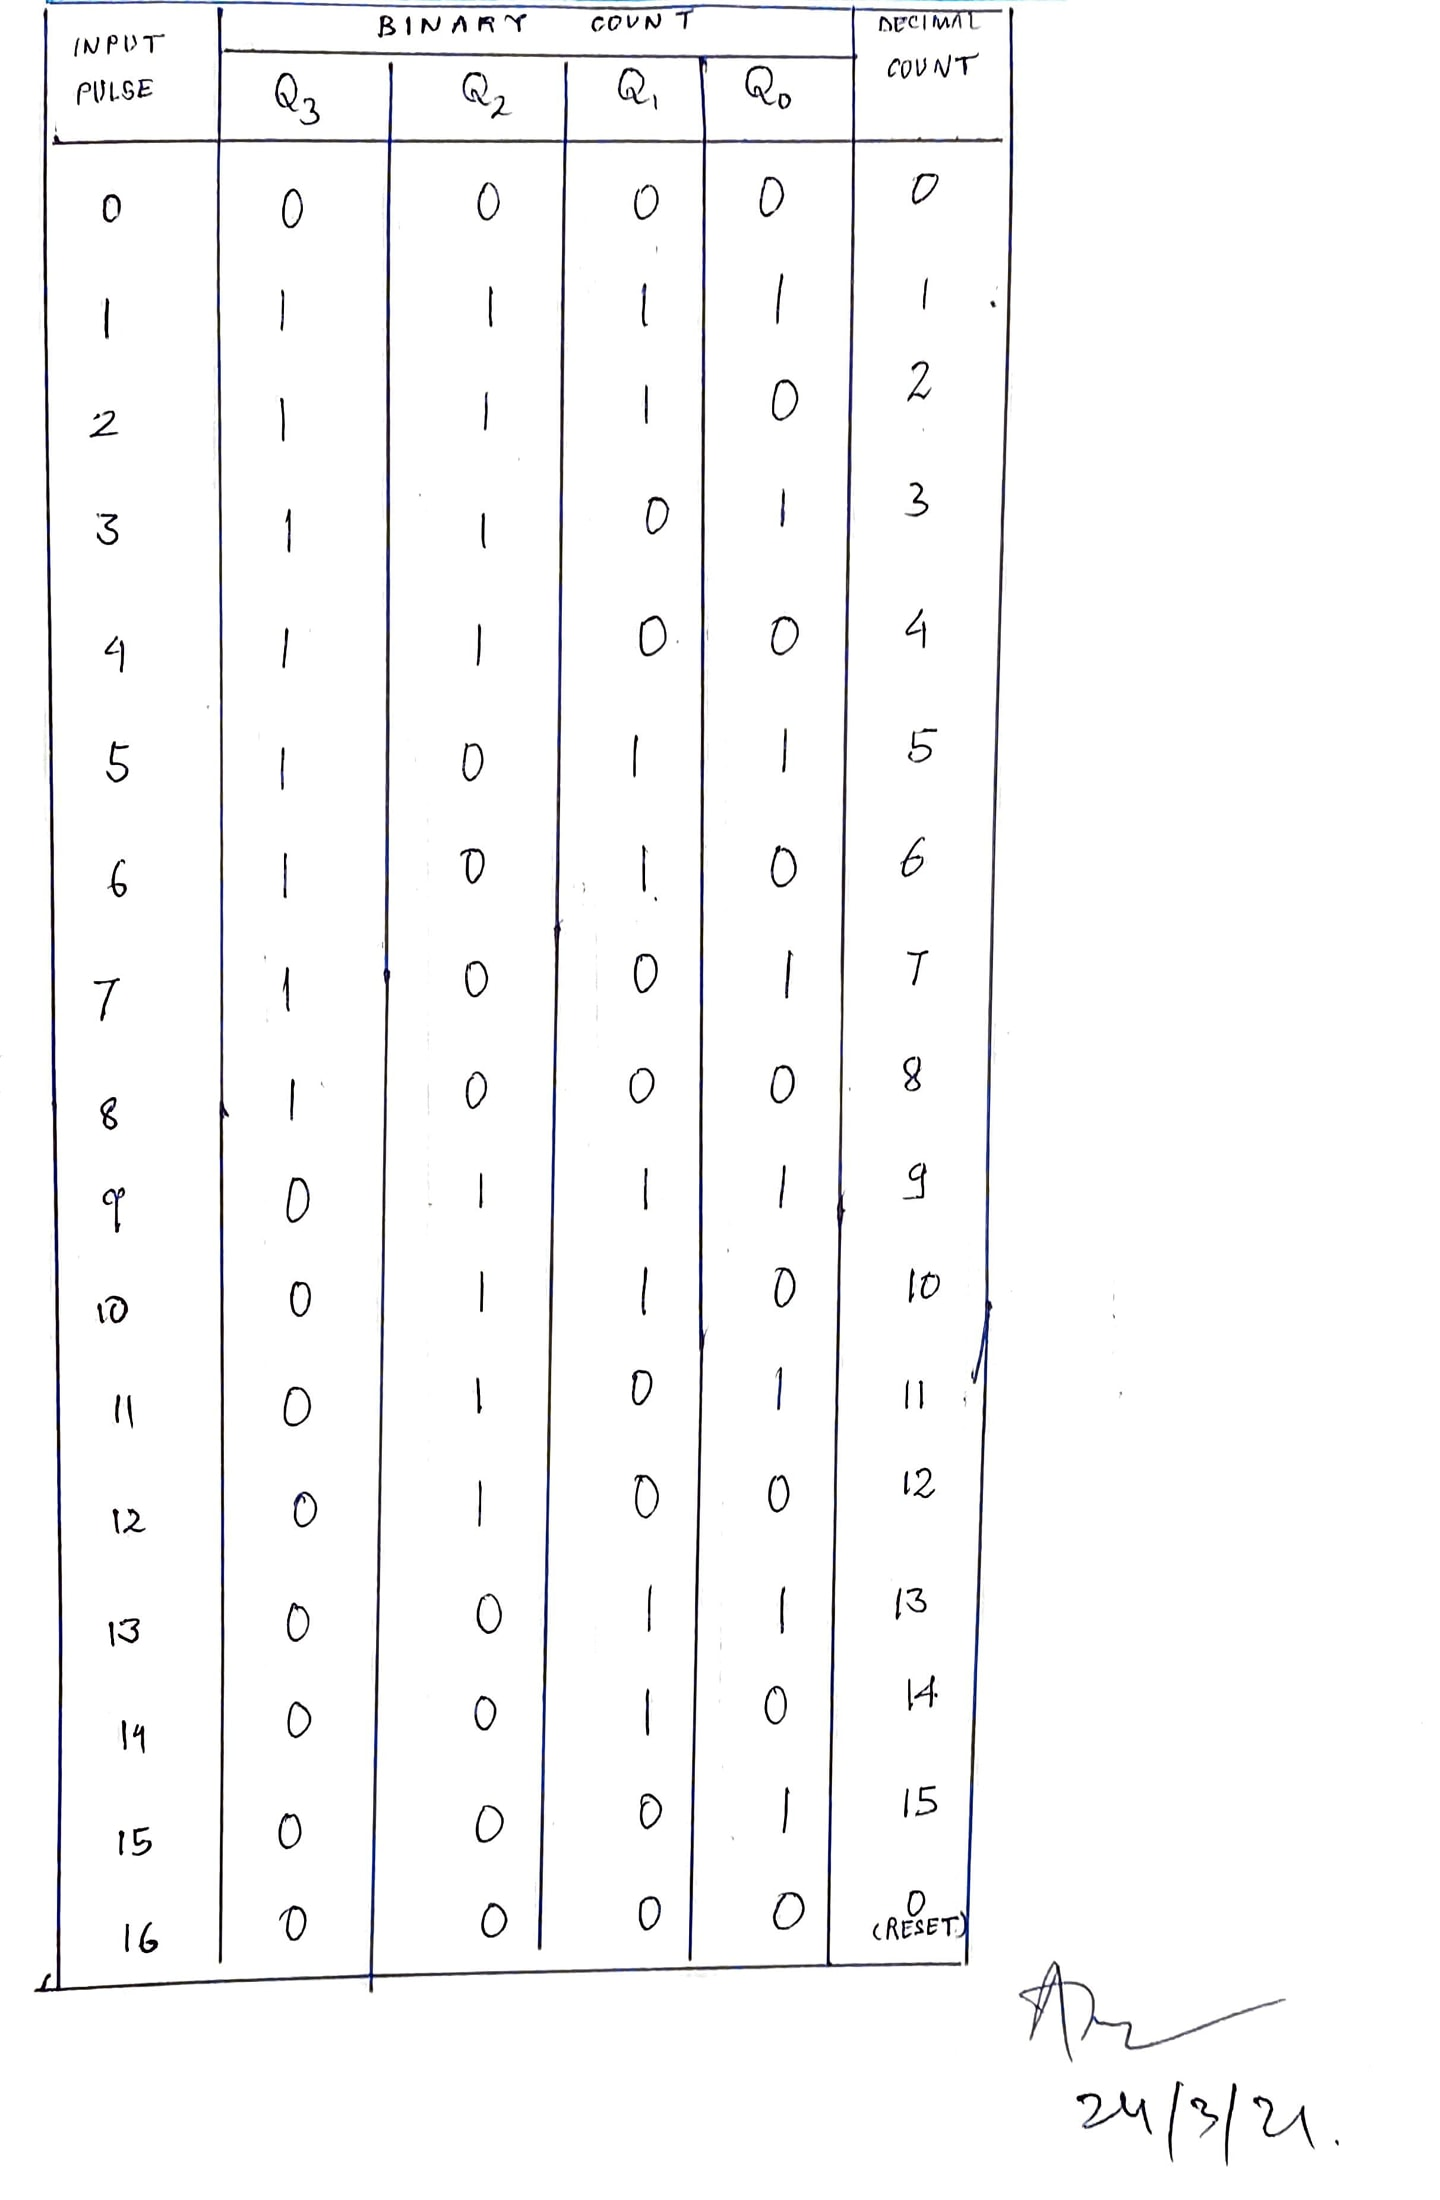
\includegraphics[scale = 0.15]{Figures/tabup_1.jpg}
\end{center}
\begin{center}
    \textbf{Characteristic table of 4-bit binary ripple down-counter}
\end{center}
\begin{center}
    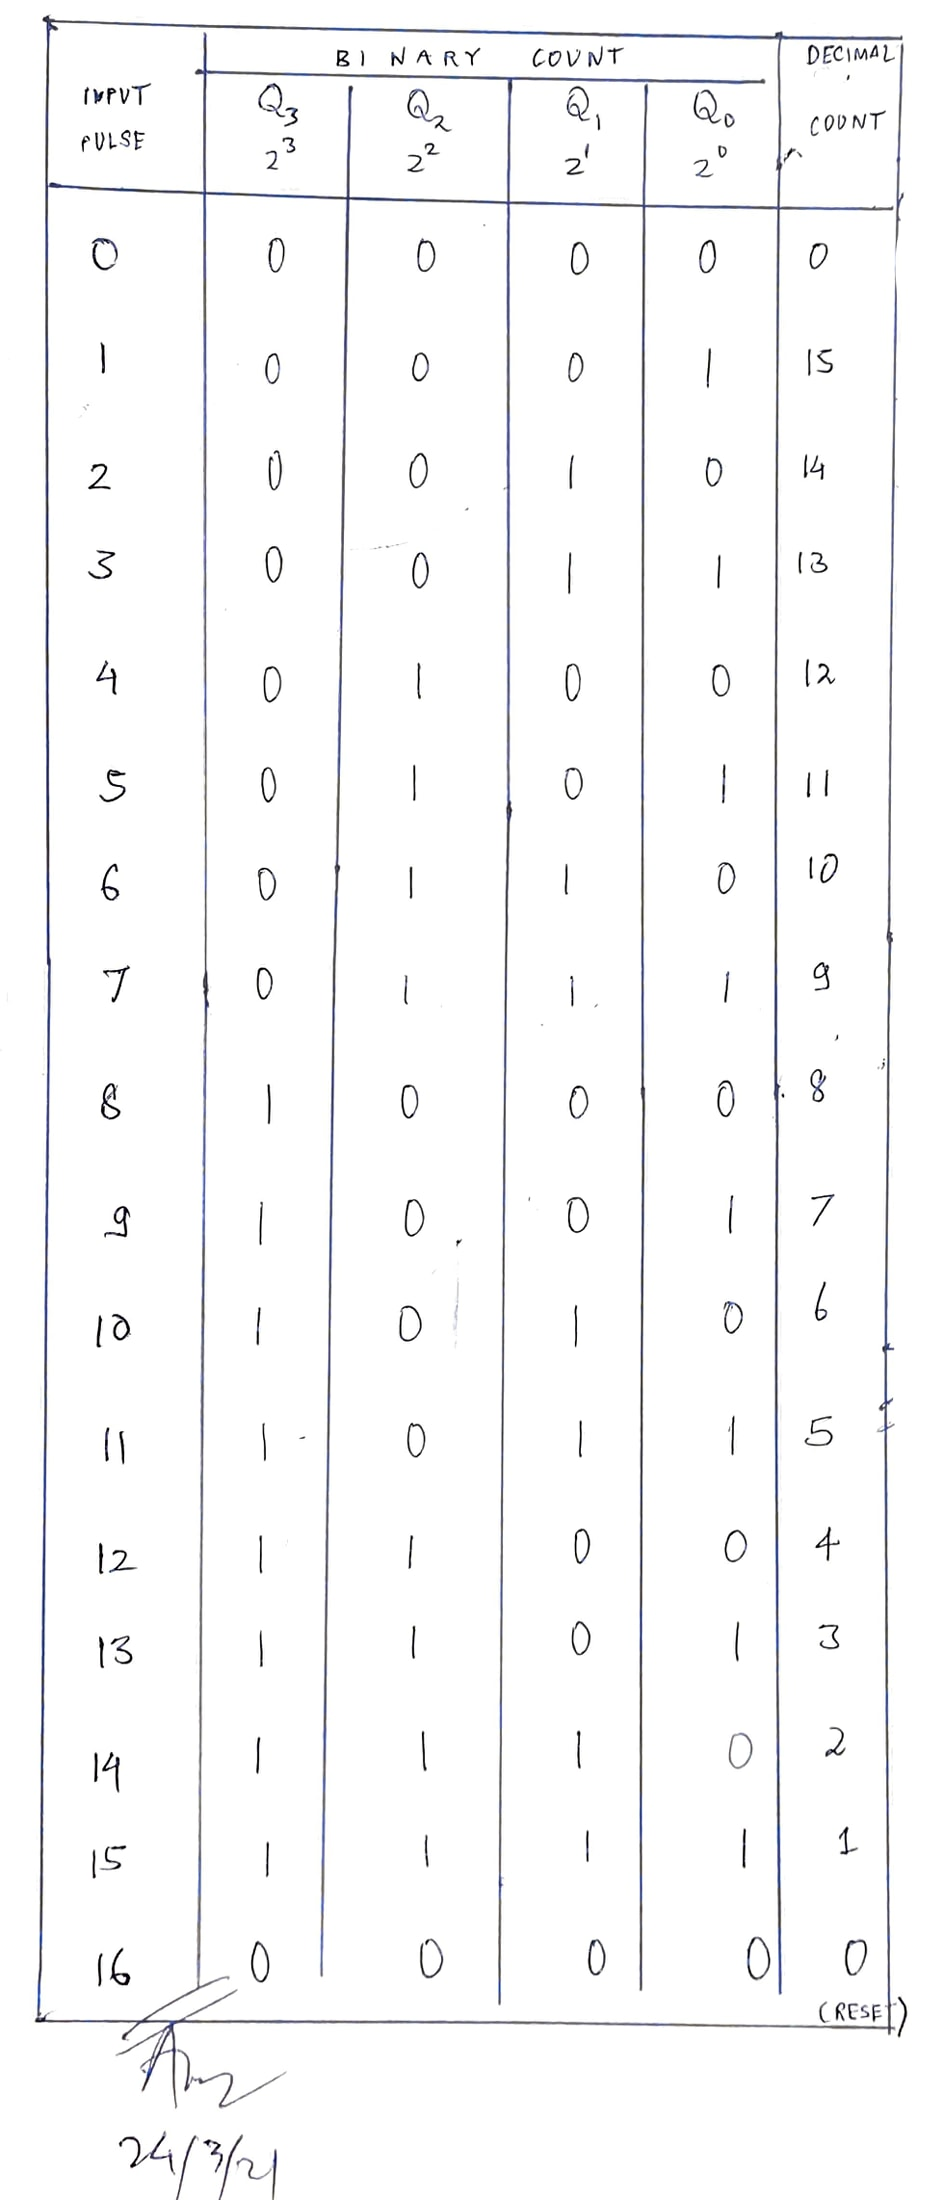
\includegraphics[scale = 0.15]{Figures/tabdown_1.jpg}
\end{center}
\begin{center}
    \textbf{Characteristic table of modulus-12 counter}
\end{center}
\begin{center}
    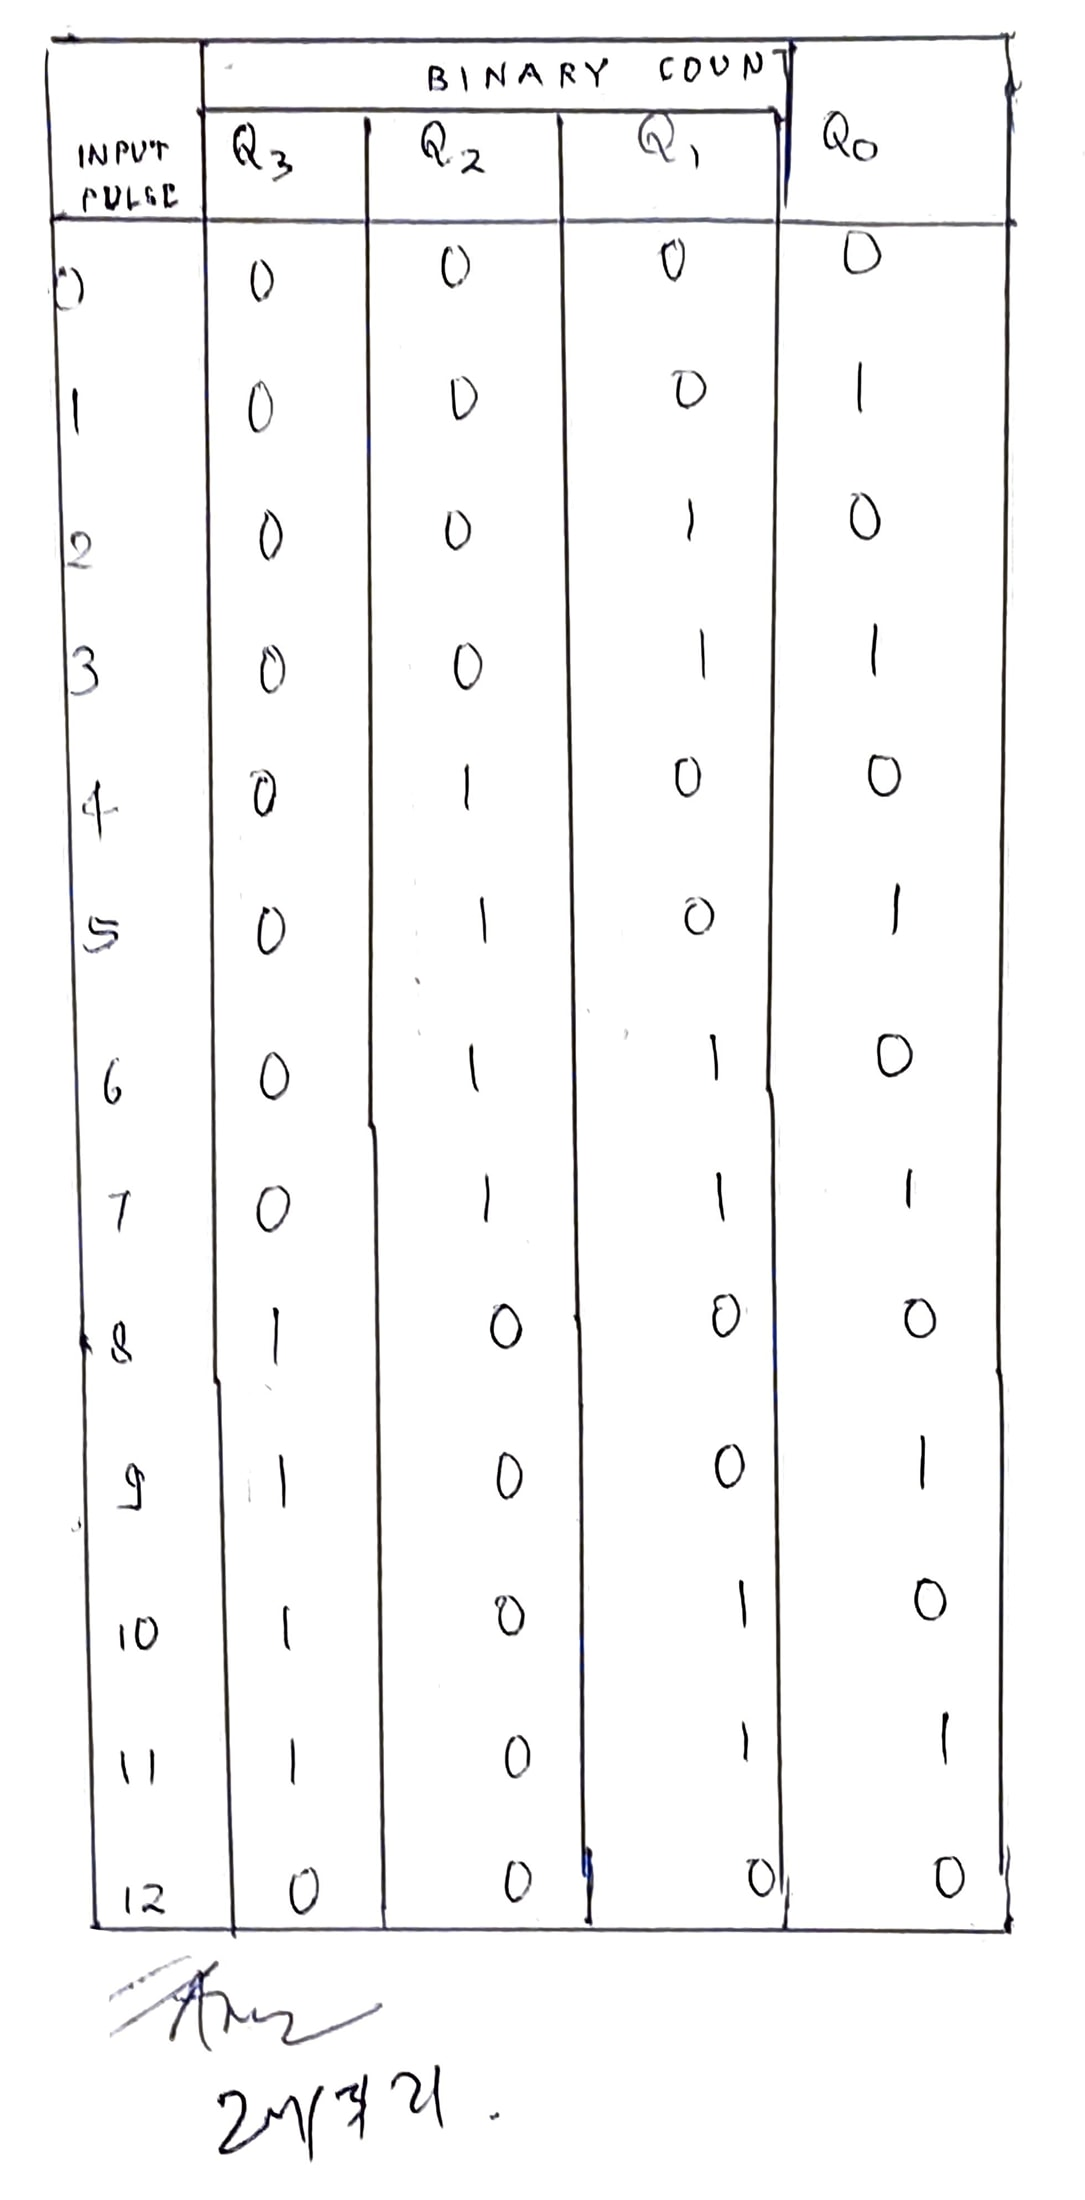
\includegraphics[scale = 0.1]{Figures/tabmod12_1.jpg}
\end{center}
\begin{center}
    \textbf{Characteristic table of ring counter}
\end{center}
\begin{center}
    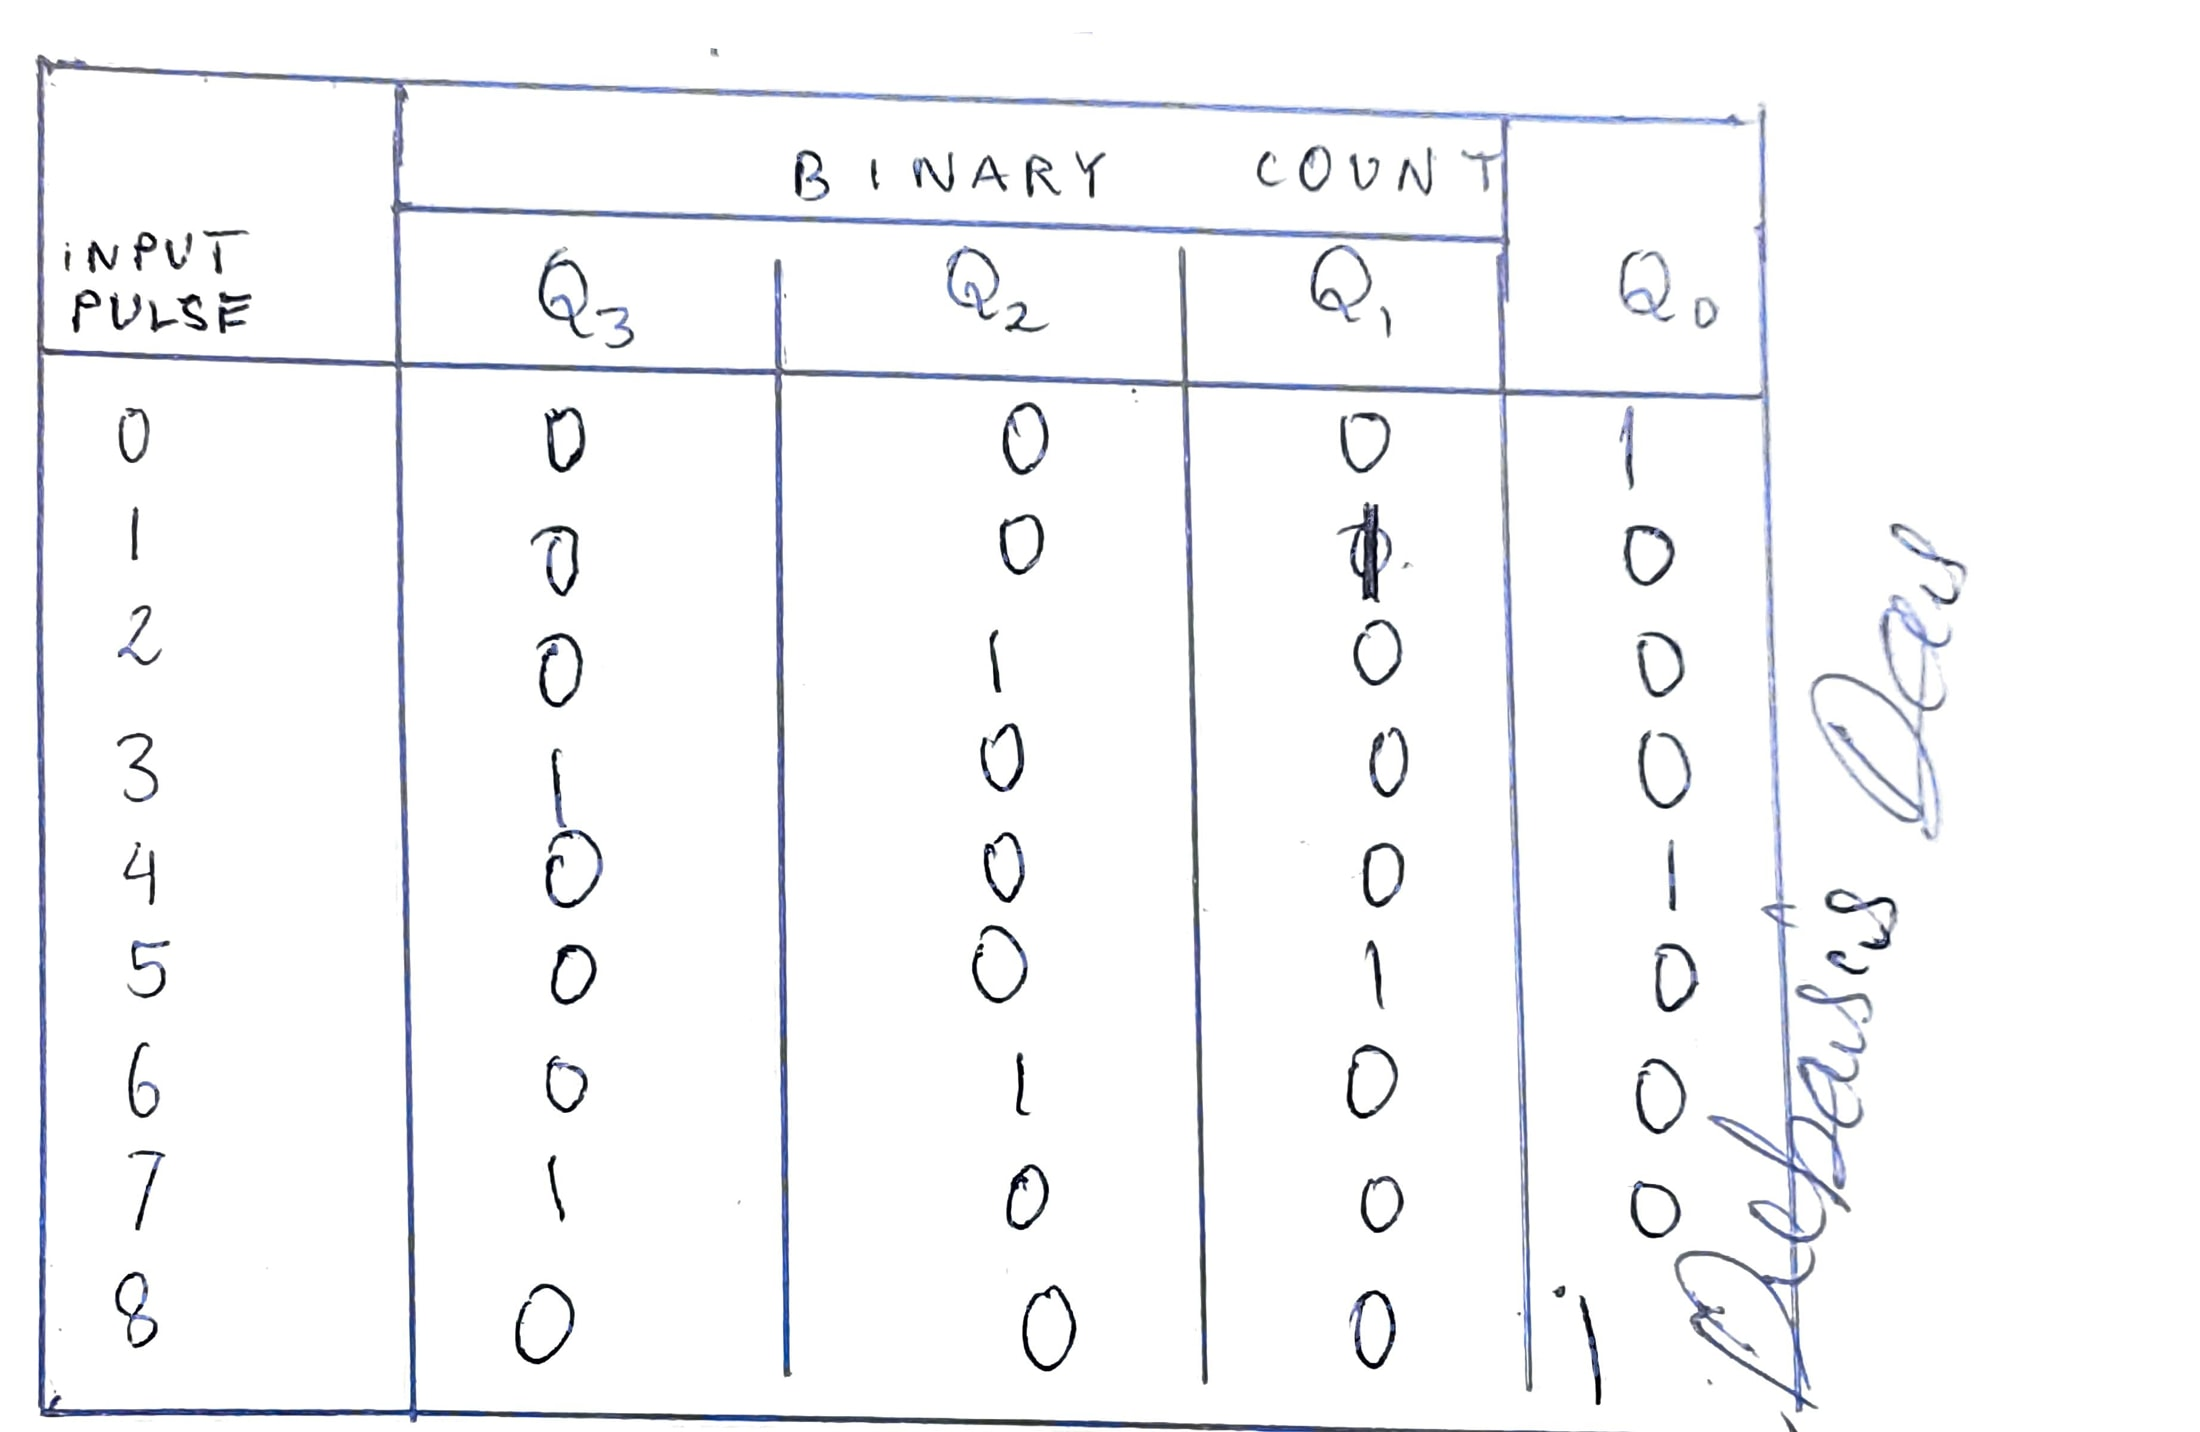
\includegraphics[scale = 0.15]{Figures/tabring_1.jpg}
\end{center}
\section{Result}
\begin{enumerate}
    \item The characteristic tables of the counters are obtained as enumerated under Observations section
\end{enumerate}
\section{Discussions}
\begin{enumerate}
    \item The working of the ripple up-counter and the ripple down counters can easily be understood by recalling flip-flops properties. When $J = K = 1$, on application of an input pulse, the output will toggle during the positive or negative edge of the pulse.
    \item The count held by this  counter is read in the reverse order from the order in which the flip-flops are triggered.  Thus, output $Q_3$ is the highest order of the count, while output $Q_0$ is the lowest order. The  binary count held by the counter is then $Q = Q_3Q_2Q_1Q_0$.
    \item The step-by-step process can be explained as: When the trailing or negative end of the first pulse arrives, the first flip-flop gives an output $Q_0 = 1$, which does not affect the second flip-flop and the counter reads 0001. On supplying 15th pulse the counter reads 1111 (decimal 15). The next clock pulse after count 1111 will cause the counter to try to increment to 10000 (decimal 16). However, that 1 bit is not held by any flip-flop and is therefore lost. As a result, the counter actually reverts to 0000, and the count begins again.
    \item For the ripple down counters, the complement output toggles at each negative edge of the clock pulse (1 to 0 transition), which is equivalent to a normal output toggling for positive edge of the clock pulse (0 to 1 transition). The counter starts from 1111 with the first pulse after it is reset and reverts back to 0000 after 15 pulses. 
    \item Although we have constructed the up and down counters separately in this experiment, we can also construct a combined up-down counter circuit.
    \item For the modulo-12 counter to work, the 4-input NAND feeds a reset pulse to the counter during state 12 (1100) and immediately after state 11 (1011). The flip-flops are reset and the counter starts counting again.
    \item In the ring counter, in the array of coupled flip-flops the last flip-flop is coupled back to the first. If one of the flip-flops is in the SET (or 1) state and the others are in the RESET (or 0 state) and then applying clock pulses, the logic 1 will advance by one flip-flop around the ring for each pulse. The logic 1 will return to the original flip-flop after exactly 4 clock pulses (shown in shades) for a 4-bit ring counter.
    \item Counters find a lot of applications in digital electronics. Most important example is that of frequency division, For frequency division, toggle mode flip-flops are used in a chain as a divide by two- counter. One flip-flop will divide the input clock frequency by 2, two flip-flops will divide it by 4 (and so on). The final  output clock signal will have a frequency value equal to the input clock frequency divided by the mod number of the counter. Such circuits are known as \emph{divide-by-n} counters, where \emph{n} is the number of counter stages used.
    \item Counters can also be used in the manufacturing of digital clocks (especially alarm clocks), time measurement, analogue to digital conversions and digital triangular wave generators.
\end{enumerate}
\section{Error Analysis}
\begin{enumerate}
    \item This experiment being a qualitative one, there are no errors per se.
    \item But we can note some precautions such as loose wiring leading to flickering of the LEDs (thus no conclusive "ON" or "OFF" inference.)
\end{enumerate}
\section{Conclusion}
\begin{enumerate}
    \item All results obtained are in accordance to the expectations.
    \item Loose connections might pose a problem while changing the \emph{enabler} and input keys between the two states.
\end{enumerate}